% !TEX root = ./report.tex

\clearpage
\section{The Inliner}
\label{scheme:start}

\todo[inline]{Introduce section with how the RVSDG helps with the different
steps in the below enumerated list.}

The inliner of this project performs the following when given an RVSDG as input:

\begin{enumerate}

	\item Scan through the RVSDG, finding all $\phi$-regions.

	\begin{enumerate}
		\item If no $\phi$-regions are found, jump to Step~\ref{ScanForApplyNodesItem}.

		\item If $\phi$-regions are found, use the approach described
in Section~\ref{sub:scheme:inlining_recur_apply_nodes} to fill a list of
\textit{loop breakers} with references to the recursive $\lambda$-nodes\
contained within the $\phi$-regions, which are \textit{not} to be
inlined.
		\label{MakeLoopBreakerListItem}
	\end{enumerate}

	\item Scan through the RVSDG, finding all the \applyNode s. Store a
reference to each in a new list.
	\label{ScanForApplyNodesItem}

	\item Order the list of \applyNode s, as discussed in
Section~\ref{sub:scheme:ordering_apply_nodes}.
	\label{OrderApplyNodesFoundItem}

	\item Look at each \applyNode~in turn in the list from
Step~\ref{OrderApplyNodesFoundItem} and decide whether or not to inline it
according to the heuristic implementation discussed in
\ref{sub:scheme:inlining_apply_nodes}.
	\label{LookAtNextCallSiteItem}

	\begin{enumerate}
		\item If the function the \applyNode~invokes is referenced in the
\textit{loop breakers} list, or if it does not meet the criteria of the inlining
heuristics discussed in Section~\ref{sub:scheme:inlining_apply_nodes}, junp to
Step~\ref{LookAtNextCallSiteItem} and evaluate the next \applyNode~in turn.

		\item If inlined, make a new list containing any newly copied (inlined)
\applyNode s.
		\label{InlineCallSiteItem}

		\begin{enumerate}
			\item If this new list is not empty, execute
Steps~\ref{OrderApplyNodesFoundItem}$\rightarrow$\ref{InlineCallSiteItem} with
this new list instead of the list from Step~\ref{ScanForApplyNodesItem}. After
list is completed, continue with previous list.
			\label{InlineNewListItem}
		\end{enumerate}

	\end{enumerate}
\end{enumerate}

\subsection{The order of call sites inlined}
\label{sub:scheme:ordering_apply_nodes}

\todo[inline]{Need reference to further ideas related to ordering of inlining.}

While implementing the inliner of this project, it came to our attention that
the order of which the functions are inlined, can have an effect on the
compiled program.

The inlining conditions we use as criteria for whether or not to inline, only
look at the properties of the function a call site invokes. Hence, when a
successive series of functions call one another, we only consider at one at a
time. Thus, the ordering of the \applyNode s we look at when deciding whether or
not to inline them, matters because inlining opportunities might be missed with
one ordering, and unveiled with another.

Figure~\ref{fig:inline_ordering_ex} illustrates the different outcomes dependent
upon the order we visit each call-site (\applyNode ). If our criteria for inlining
is that the inlined function does not exceed the inlining condition:
\textit{Statement Count} $> 4$, we can inline $\lambda_1 \Rightarrow \lambda_2
\Rightarrow \lambda_3$. However, if we inline $\lambda_3 \Rightarrow \lambda_2$,
then the combined function $\lambda_{2+3}$ will have a SC exceeding the given
limit.

\begin{figure}[H]
	\centering
	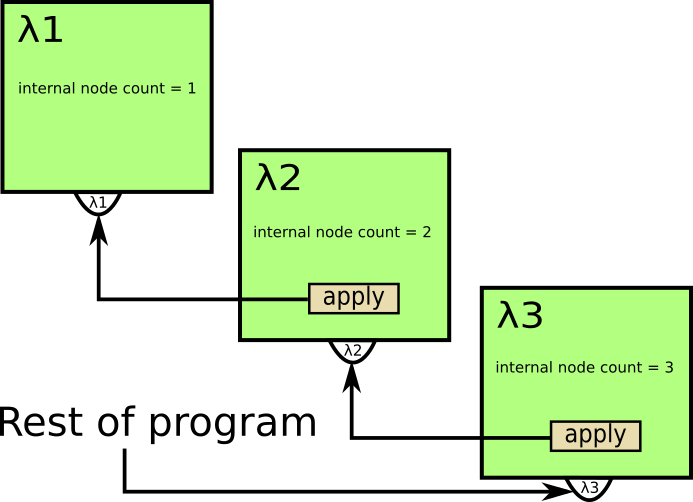
\includegraphics[width=0.75\textwidth]{figures/inline_ordering_ex}
	\caption{A minimal example of an RVSDG subgraph, showing why the ordering of
inlining makes a difference for the resulting program executable.}
	\label{fig:inline_ordering_ex}
\end{figure}

\subsection{Inlining a call site}
\label{sub:scheme:inlining_apply_nodes}

Utilizing the \textit{inlining conditions} described in
Section~\ref{sub:meth:inlining_conditions}, heuristics evaluating the function
invoked by each \applyNode can be written in \textit{Conjunctive Normal Form}
(CNF). This enables an efficient way to search the parameter space for optimal
parameters for the inlining heuristics.

The inliner evaluates each \applyNode~with the given heuristic, and decides
whether or not to inline the call site this \applyNode~represents, depending on
the properties of the function it invokes.

\todo[inline]{Describe the algorithm and inliner conditions we land on after
testing.}

\unsure[inline]{Is the below paragraph too implementation specific?}

When a function is inlined, additional \applyNode s might be copied into the
RVSDG. These are handled as discussed in Step~\ref{InlineNewListItem}. However,
when inlining a call-site, the optimization of an RVSDG performed after each
inlining might also remove previously found \applyNode s. Hence, care must be
taken with any list of references to found \applyNode s not yet evaluated by the
heuristic.

\subsection{Deciding which recursive functions to inline}
\label{sub:scheme:inlining_recur_apply_nodes}

The inliner evaluates all functions, recursive or not, with the same heuristic,
described in Section~\ref{sub:scheme:inlining_apply_nodes}. However, the inliner
of this project only evaluates \textit{some} of the \applyNode s invoking
recursive functions, to ensure termination of the compiler.

\todo[inline]{Describe how we decide which recursive functions we evaluate with
the inlining heuristic.}

The inliner of this project performs the following when given an RVSDG as input:

\begin{enumerate}
	\item If $\phi$-regions are found, use Tarjan's \textit{Strongly Connected
Component} (SCC) algorithm\cite{doi:10.1137/0205051} to find any SCCs within
each $\phi$-region.

	\begin{enumerate}
	\item If there exist any $\lambda$-nodes which are not part of any SCC in
the $\phi$-region, add a reference to each and all of these to the list of
\textit{loop breakers}, ref. Step~\ref{MakeLoopBreakerListItem} from
Section~\ref{scheme:start}.

	\item If any $\lambda$-nodes are found to be part of an SCC in the
$\phi$-region, \todo{Explain how when implemented}select one these per SCC to be
a \textit{loop breaker}, and add a reference to each of the loop breakers to the
list of \textit{loop breakers}.
	\end{enumerate}
\end{enumerate}

Hence, the inliner has a list of recursive functions which it knows \textit{not}
to inline, to ensure termination of the compilation. All other remaining
recursive functions may then be safely inlined with the same criteria as any
non-recursive functions.
